%!TEX root=TFG-book.tex
	

	
	%	En los mismos términos, F se considera continua en $x_0 \in D \iff \exists \lim_{x \rightarrow x_0} F(x)$ y además:
	%	\[\lim_{x \rightarrow x_0} F(x) = F(x_0)\]
	%	Además, si es continua en todo punto de D, se dice que es continua en D y se escribe $F \in \mathcal{C^0}(D)$.
	%	\end{definition}

\chapter{Métodos directos}


Un sistema de ecuaciones no lineales:

$$\begin{cases}
	f_1(x_1,...,x_n)  = 0 \\
	f_2(x_1,...,x_n)  = 0 \nonumber \\
	...                   \nonumber \\
	f_n(x_1,...,x_n)  = 0 \nonumber
\end{cases}$$

donde podemos considerar la función $f_i$ como mapeo del vector $x = (x_1,...,x_n)$ del espacio dimensional $\mathbb{R}^n$ en la recta real $\mathbb{R}$. Este sistema también se puede representar como una única función de $\mathbb{R}^n$ en $\mathbb{R}^n$:
\[F(x_1,...,x_n) = (f_1(x_1,...,x_n),...,f_n(x_1,...,x_n))\]
Empleando una notación vectorial, de forma que podemos escribir el sistema como:
\[F(x) = 0\]

\section{Puntos fijos para funciones de varias variables}

% Tomamos D cerrado porque sino tendríamos que definir los puntos que tienen límite como los de D' de su conjunto de acumulación o clausura

	Recordemos que dada $F: D \subset \mathbb{R}^n \longrightarrow \mathbb{R}^m$, donde su dominio D es un conjunto cerrado, de forma que la función $f$ es contractiva en D, se dice que tiene límite $L \in  \mathbb{R}^m$ en $x_0 \in D$ y se escribe:
	\[\lim_{x \rightarrow x_0} F(x) = L\]
	si dado $\epsilon > 0$, existe un $ \delta > 0$ tal que para todo
	$ x \in D$:
	 $$0 < \|x-x_0\| < \delta \Rightarrow ||f(x) - L|| < \epsilon $$
	La existencia de límite es independiente de la norma vectorial que se use. 
	%El valor $\delta$ es independiente de la norma.

%	\begin{definition}
	%	Sea $f: D \subset \mathbb{R}^n \longrightarrow \mathbb{R}$. Se dice que es continua en $x_0 \in D$ siempre que $\exists \lim_{x \rightarrow x_0} f(x)$ y además:
	%	\[\lim_{x \rightarrow x_0} f(x) = f(x_0)\]
	%	Además, si es continua en todo punto de D, se dice que es continua en D y se escribe $f \in \mathcal{C^0}(D)$.	
	%	\end{definition}

Para poder estudiar de forma sencilla el límite de funciones en varias dimensiones, es más sencillo estudiar el límite para cada una de las componentes:

\begin{proposition}
	Sea $F: D \subset \mathbb{R}^n \longrightarrow \mathbb{R}^m$ de la forma $F(x) = (f_1(x),...,f_m(x))$, donde $f_i: D \subset \mathbb{R}^n \longrightarrow \mathbb{R}^m$, $1 \leq i \leq m$. Entonces el límite:
	\[\lim_{x \rightarrow x_0} F(x) = L = (L_1,...,L_m) \iff \lim_{x \rightarrow x_0} f_i(x) = L_i, 1 \leq i \leq m\]
\end{proposition}

%	\begin{definition}
	
% Introduccion

\begin{definition}
	Se dice que una función $G$ de $D \subset \mathbb{R}^n$ tiene un punto fijo en $p \in D$ si $G(p) = p$.
\end{definition}

Generalmente podemos encontrarnos las ecuaciones de la forma $f(x) = 0$, que no es más que otra forma de escribir el sistema como $f(x) = G(x) - x = 0$. Para transformar de forma inversa, podemos sumar un término $x$ a ambos lados de la ecuación, o alternativamente despejar el término $x$ si aparece de forma independiente en la ecuación $f(x)$ original. De esta forma, observamos que si la función $G$ tiene un punto fijo, entonces la función $f$ posee un cero en ese mismo punto. \\

El método del punto fijo es un método iterativo, también denominado método de aproximaciones sucesivas. Dado un valor inicial $x_0$, tomamos un esquema iterativo que cumple que cada punto $x_i$ es la imagen $G(x_{i+1})$ del punto anterior. Este método nos acerca sucesivamente al valor $x = G(x)$ con una cota de error predeterminada, siempre que $G$ sea continua y $x_i \longleftrightarrow x$ converjan a un punto fijo. \\

% CTRL + t para comentar
% CTRL + u para descomentar

%\begin{theorem}
%	Sea $f$ una función de $D \subset \mathbb{R}^n$ en $\mathbb{R}$, y $x_0 \in D$. Si existen constantes $\delta > 0$ y $K > 0$, con
%	\[\left| \frac{\partial f(x)}{\partial x_j}  \right| \leq K, j = 1 ,..., n\]
%	siempre que $||x-x_0|| < \delta$ y $x \in D$, entonces $f$ es continua en $x_0$.

%\end{theorem}

 Vamos a ver que siempre se pueden encontrar una solución a la ecuación del punto fijo bajo ciertas condiciones:

\begin{theorem}[Teorema de existencia de punto fijo]
	Sea $$D = \{(x_1,...,x_n) , a_i \leq x_i \leq b_i, \forall i = 1 ,..., n\}$$ para algún conjunto de constantes $a_1$, ..., $a_n$ y $b_1$, ..., $b_n$. Si $G : D \subset \mathbb{R}^n \longrightarrow \mathbb{R}^n$ es una función continua tal que $G(D) \subseteq D$ y es lipschitziana de constante $0<K<1$, entonces la sucesión $\{x_{k}\}_{k \in \mathbb{N}}$ dada por $x_{0} \in D$ y generada por:
	\[x_{k} = G(x_{k-1} )\ \forall k \geq 1\]
	converge en un único punto fijo $p \in D$ y además:
	\[||x_{k} - p|| \leq \frac{K^k}{1-K}||x_{1} - x_{0}|| \]
\end{theorem}

\begin{proof}
	Como $G$ es lipschitziana, tenemos que:
	\begin{align*}
	|| x_{k} - x_{k-1} || & = || G(x_{k-1}) - G(x_{k-2}) || \leq K || x_{k-1} - x_{k-2} || \\
	& \leq K^2|| x_{k-2} -  x_{k-3} || \leq \ldots \leq K^{k-1}|| x_{1} - x_{0} ||
	\end{align*}

	Veamos que $\{x_{k}\}$ es una sucesión de Cauchy: \\
 	Como $D$ está acotado, podemos tomar un $r > 0$ con $||x_{1} - x_{0}||\leq r(1-K) \leq r$, pues $0 < K < 1$. Tomaremos esta cota únicamente para simplificar el resultado. \\
 	Dado $m>l$, entonces:

	\begin{align*}
	||x_{m}-x_{l}||& \leq ||x_{m} - x_{m-1}|| + ||x_{m-1} - x_{m-2}|| +  \ldots+||x_{l+1} -  x_{l}||\\
	& \leq (K^{m-1} + K^{m-2} + \ldots + K^l) (1-K)r \\
	\end{align*}
	Resolvemos esta serie geométrica y acotamos convenientemente:
	\begin{align*}
	\sum_{i = k-1}^{l} K^{i} = K^{l} \sum_{i = 0}^{m-1-l} K^{i} = K^{l}\frac{1-K^{m-l}}{1-K} < \frac{K^{l}}{1-K}
	\end{align*}
	\begin{align*}
	||x_{m}-x_{l}|| < \frac{K^{l}}{1-K} ||x_{1}-x_{0}|| < K^{l} r
	\end{align*}

	Por lo tanto, como $K<1$, podemos hacer $K^lr$ arbitrariamente pequeño para $l$ suficientemente grande.
	
	Con esto hemos visto que $\{x_{k}\}$ es sucesión de Cauchy, luego converge a un $p$ en el espacio completo $\mathbb{R}^{n}$. Como $D$ es cerrado y $x_{k} \in D$, $\forall$ $k$, $p \in D$.
	
	Por último:
	
	\[||x_{k}-p|| = \lim_{m \to \infty} ||x_{m}-x_{k}|| \leq \frac{K^l}{1-K}||x_{1}-x_{0}||\]
\end{proof}

\subsection{Algoritmo del punto fijo para sistemas}

Para programar el método podemos seguir las siguientes instrucciones: 

\begin{itemize}
\item INPUT número n de ecuaciones ; aproximación inicial $x_0$ 
\item TOL número máximo de iteraciones N 
\item Paso 1	Sea k = 1, entonces $x = x_0$ 
\item Paso 2 Cuando ($k \leq N$) hacer pasos  3 al 6 
\item Paso 3 Resolver el sistema de punto fijo x = f(x) 
\item Paso 4 Si $||x|| < TOL $ entonces OUTPUT (x) (El proceso tuvo éxito). STOP 
\item Paso 5 Sea k = k+1 
\item Paso 6 OUTPUT ('Número máximo de iteraciones excedido') (El proceso no tuvo éxito). STOP.
\end{itemize}


Hemos programado el método anterior en SAGE mediante el siguiente código:

\begin{minted}{python}
def MetodoPuntoFijo(f,x0,n):
	x = x0
	for k in [1..n]:
	x = f(*x)
	return x
\end{minted}

O alternativamente, si queremos ver todos los pasos intermedios:
\begin{minted}{python}
def MetodoPuntoFijoIteraciones(f,x0,n):
	x = [x0] + [0]*n
	for k in [1..n]:
	x[k] = f(*x[k-1])
	return x
\end{minted}

\subsection{Ejemplos}

A continuación ilustraremos el método en algunos ejemplos. \\
En primer lugar, consideraremos el método en una dimensión, pues será más sencillo representarlo. \\
Vamos a tomar $cos(x)$ como primer ejemplo. Sabemos que restringido al intervalo $D = [0,\pi]$, el coseno es contractivo, por tanto estamos dentro de las hipótesis del teorema:

\begin{example}
	$$f(x) = \frac{cos(x)}{2}$$
	
	Como sabemos $cos(x)$ es infinitamente diferenciable, tiene un máximo absoluto en cada una de las derivadas dentro del intervalo cerrado D. Por el teorema del valor medio podemos observar que ese máximo nos vale como constante de Lipschitz.
	
	Tomamos $x_0 = 0.5$ y procedemos a aplicar el método.
	Si hacemos 20 iteraciones, obtenemos el valor $x = 0.739006779780813$ como aproximación del punto fijo.
	
	Para escribir en SAGE definimos como:
	\begin{minted}{python}
		f(x)=(cos(x),)
		MetodoPuntoFijo(f,(0.5,),20)
	\end{minted}
Ya que estamos definiendo el método de forma vectorial.\\

Y la gráfica de la función junto a la recta y=x, que cortan en el punto fijo, junto a las líneas verdes que indican cada una de las iteraciones:

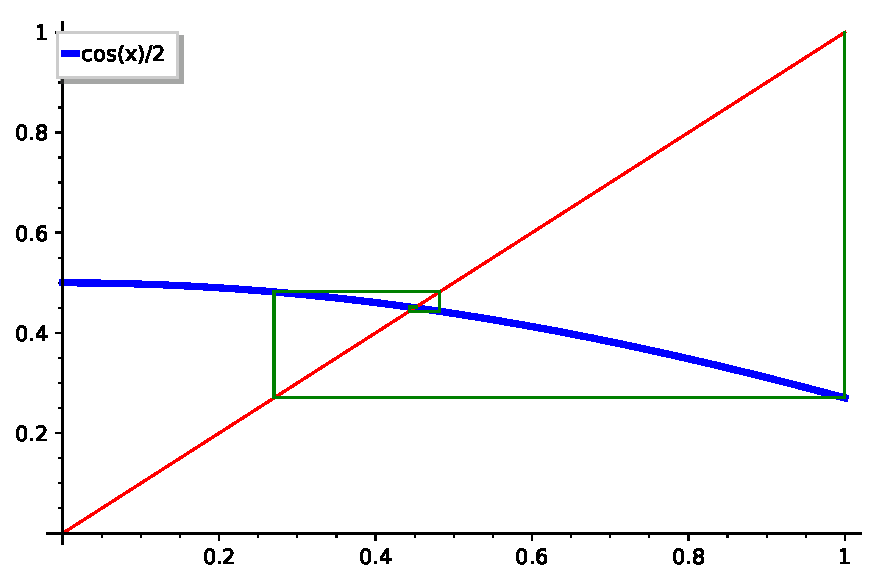
\includegraphics[scale=1]{ejemplo1_puntofijo}
\end{example}

A continuación vamos a introducir un contraejemplo para ver que no todas las funciones contractivas tienen punto fijo:

\begin{example}
$$h(x) = 1+log(1+ exp(x)) $$

Esta función es claramente contractiva, pues si derivamos:
$$|h'(x)| = \frac{e^{x}}{1+e^{x}} < 1$$
Pero para todo $x \in D$, tenemos que $|h(x)-x| > 1$, por lo cual no va a tener un punto fijo.\\

Podemos aplicar el método don 20, 100 y 200 iteraciones. Como podemos observar, los resultados serán $21.1726982050075$, $101.172698206017$ y $201.172698206017$, que no converge a ningún punto, sino que crece indefinidamente. Vamos a verlo gráficamente:


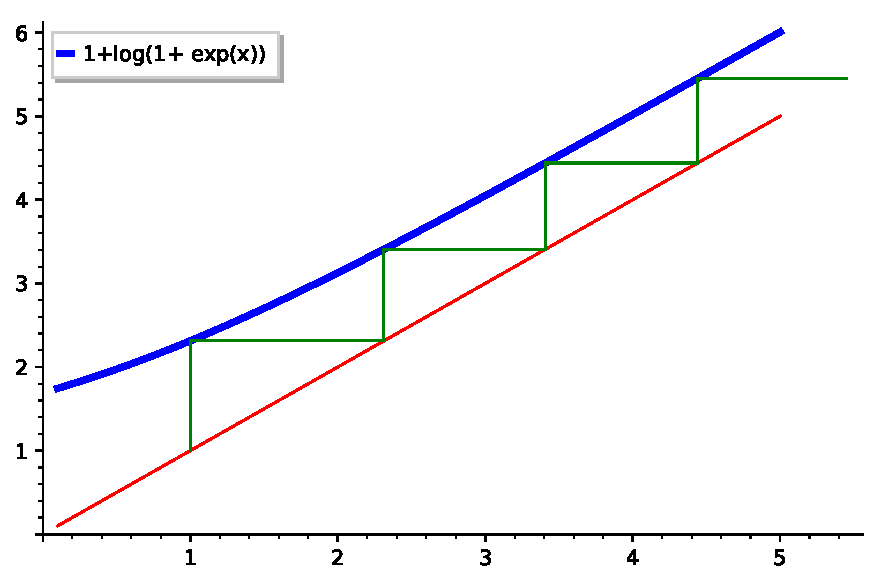
\includegraphics[scale=1]{ejemplo2_puntofijo}

Es claro entonces, pues nuestra función tiene una asíntota en $y=x$. Por eso nunca converge a un punto fijo, pues no se llegan a cortar ambas funciones.


\end{example}

El siguiente ejemplo será bidimensional, para que podamos observar cómo funciona el método en dimensiones superiores:

\begin{example}
	$$m(x,y) = (\frac{1}{e^{x}},\frac{1}{e^{y}})$$
Lo implementamos en SAGE como:
\begin{minted}{python}
	MetodoPuntoFijo(m,(0.5,0.5),10)
\end{minted}

Vemos que con pocas iteraciones el método converge al punto $(0.5669072, 0.5669072)$.

\end{example}

Por último, un ejemplo bidimensional donde no converge el método del Punto Fijo:
\begin{example}
$$
\begin{matrix}
	g_1(x,y) & = x^2+xy-10 \\
	g_2(x,y) & = y + 3xy^2 - 57 \\
	G(x,y)   & = (g_1(x,y),g_2(x,y))
\end{matrix}
$$

Tomamos el punto inicial $(0.5,0.5)$. Si observamos cada iteración podemos ver que esta función no se va aproximando a ningún punto fijo:

\begin{minted}{python}
[(0.500000000000000, 0.500000000000000),
(-9.50000000000000, -56.1250000000000),
(613.437500000000, -89888.5703125000),
(-5.47647242846680e7, 1.48696422300132e13),
(-8.14328857763300e20, -3.63264701075255e34),
(2.95816929092346e55, -3.22379544959185e90),
(-9.53653269920141e145, 9.22314921617083e236),
(-8.79568640896269e382, -2.43371784625526e620),
(2.14062189835574e1003, -1.56290091483395e1624),
(-3.34557992325377e2627, 1.56864297681102e4252),
(-5.24802044997198e6879, -2.46968112630275e11132)]
\end{minted}

	
\end{example}
                                           
%\subsection{Aceleración de la convergencia}
%
%Una forma de acelerar la convergencia en la fórmula del punto fijo es usar la última estimación $x_1^{(k)}$,...,$x_{i-1}^{(k)}$, en lugar de $x_1^{(k-1)}$,...,$x_{i-1}^{(k-1)}$ para computar $x_i^{(k)}$ como lo haríamos en el método de Gauss-Seidel de sistemas lineales.

\subsection{Importancia del método}

La gran importancia del Teorema del Punto Fijo deriva de varios factores. Primero de la existencia y unicidad de solución; De la posibilidad de hallar un error a priori y a posteriori; De ser un método convergente iterativo donde podemos conocer la velocidad de convergencia; Y por último de la estabilidad del método, ya que un cambio en el punto inicial no varía el límite de iteraciones.

\section{Método de Newton}

Consideramos el sistema $$F(x)=0$$ donde $F: D \subset \mathbb{R}^{n} \longrightarrow \mathbb{R}^n$ es una función de clase $\mathcal{C}^{2}$ y $p \in D$ es solución, es decir $F(p) = 0$.
Vamos a transformarlo en un problema de punto fijo $$G(x) = x$$ con G una función de la forma:
\[G(x) = x - A(x)^{-1} F(x)\]
descritos en el apartado anterior, donde cada $x_{i} \in A(x) \subset M_{n}$. El objetivo será elegir A(x) de modo que se verifique el siguiente teorema, que asegura una convergencia cuadrática del método del punto fijo:\\
%En esta sección vamos a escribir $G$ como una serie de Taylor en n variables alrededor del punto $p$.

\begin{theorem}\label{TPF}
	Sea $G : \mathbb{R}^n \to \mathbb{R}^n$ diferenciable y $J_G$ su matriz jacobiana.
	Si $p$ es un punto fijo de $G$ y $||J_G(p)|| = \sigma < 1$, entonces existe un entorno abierto $N$ de $p$ tal que la sucesión definida por $x^{(k)}=G(x^{(k-1)})$ con $x^{(0)}\in N$ converge a $p$.
\end{theorem}
\begin{proof}
Como $G$ es diferenciable, para todo $\epsilon > 0$ existe un $\delta > 0$ tal que:

\[ ||G(x) - G(p) - J_G(p)(x-p) || \leq \epsilon ||x-p|| \]

cuando $x \in N_\delta(p)=\{x : ||x-p||<\delta\}$. Por lo tanto, para cualquier $x \in N_\delta(p)$:

\[ ||G(x)-G(p)|| \leq ||G(x) - G(p) - J_G(p)(x-p)|| + ||J_G(p)(x-p)|| \leq (\epsilon+\sigma) ||x-p|| \]

Tomando $\epsilon$ suficientemente pequeño, tenemos entonces que para $\alpha=\epsilon+\sigma<1$. Luego si $x^{(0)} \in N_\delta(p)$, entonces:

\[ ||x^{(1)}-p|| = ||G(x^{(0)})-G(p)|| \leq \alpha ||x^{(0)} - p|| \]

Luego $x^{(1)} \in N_\delta(p)$. Sigue por inducción que $x^{(k)} \in N_\delta(p)$ para todo $k$ y además:

\[ ||x^{(k)}-p|| \leq \alpha ||x^{(k-1)}-p|| \leq \dots \leq \alpha^k ||x^{(0)}-p|| \]

Luego $x^{(k)}$ tiende a $p$ cuando $k \to \infty$.
\end{proof}

\subsection{Matriz Jacobiana}

Supongamos que nuestra matriz $A(x) \in \mathbf{M}_n$ es matriz cuadrada de valores de $\mathbb{R}^n$ en $\mathbb{R}^n$, que además es no singular cerca de la solución $p$ de $F(x) = 0$. Si llamamos $b_{ij}(x)$ a los elementos de $A(x)^{-1}$, para $G(x) = x - A(x)^{-1}F(x)$, tenemos $g_i = x_i - \sum_{j=1}^{n} b_{ij}(x)f_j(x)$. Así:
\[\frac{\partial g_{i}}{\partial x_{k}}(\mathbf{x})=\left\{\begin{array}{ll}
	1-\sum_{j=1}^{n}\left(b_{i j}(\mathbf{x}) \frac{\partial f_{j}}{\partial x_{k}}(\mathbf{x})+\frac{\partial b_{i j}}{\partial x_{k}}(\mathbf{x}) f_{j}(\mathbf{x})\right), & \text { si } i=k ,\\
	-\sum_{j=1}^{n}\left(b_{i j}(\mathbf{x}) \frac{\partial f_{j}}{\partial x_{k}}(\mathbf{x})+\frac{\partial b_{i j}}{\partial x_{k}}(\mathbf{x}) f_{j}(\mathbf{x})\right), & \text { si } i \neq k .
\end{array}\right.\]

Para aplicar el teorema anterior, impondremos que $\frac{\partial g_i(p)}{\partial x_k} = 0, \forall i \leq 1, \forall k \leq 1$. Entonces cuando $i = k$ tenemos:
\[1=\sum_{j=1}^{n} b_{i j}(\mathbf{p}) \frac{\partial f_{j}}{\partial x_{i}}(\mathbf{p})\]
Y cuando $k \neq i$:
\[\sum_{j=1}^{n} b_{i j}(\mathbf{p}) \frac{\partial f_{j}}{\partial x_{k}}(\mathbf{p})=0\]

Recordamos que la matriz jacobiana se define como:
\[J(\mathbf{x})=\left[\begin{array}{cccc}
	\frac{\partial f_{1}}{\partial x_{1}}(\mathbf{x}) & \frac{\partial f_{1}}{\partial x_{2}}(\mathbf{x}) & \cdots & \frac{\partial f_{1}}{\partial x_{n}}(\mathbf{x}) \\
	\frac{\partial f_{2}}{\partial x_{1}}(\mathbf{x}) & \frac{\partial f_{2}}{\partial x_{2}}(\mathbf{x}) & \cdots & \frac{\partial f_{2}}{\partial x_{n}}(\mathbf{x}) \\
	\vdots & \vdots & & \vdots \\
	\frac{\partial f_{n}}{\partial x_{1}}(\mathbf{x}) & \frac{\partial f_{n}}{\partial x_{2}}(\mathbf{x}) & \cdots & \frac{\partial f_{n}}{\partial x_{n}}(\mathbf{x})
\end{array}\right]\]

Imponiendo las condiciones para $k = i$ y para $k \neq i$, obtenemos:
\[A(p)^{-1}J(p) = Id \Rightarrow A(p) = J(p)\]

Entonces podemos decir que una opción para aproximar A(x) puede ser la matriz Jacobiana.

El método de Newton para sistemas no lineales quedaría como:
\[\mathbf{x}^{(k)}=\mathbf{G}\left(\mathbf{x}^{(k-1)}\right)=\mathbf{x}^{(k-1)}-J\left(\mathbf{x}^{(k-1)}\right)^{-1} \mathbf{F}\left(\mathbf{x}^{(k-1)}\right)\]

Estudiemos la convergencia de este método. Para ello, nos será útil el siguiente lema:

\begin{lemma}
Sea $F : \mathbb{R}^n \to \mathbb{R}^n$ diferenciable y sea $J$ su matriz jacobiana. Si $J$ es lipschitziana de constante $\gamma$  en un conjunto convexo $D$, entonces para todo $x,y \in D$:
\[ || F(y)-F(x)-J(x)(y-x) || \leq \frac{1}{2} \gamma ||x-y||^2 \]
\end{lemma}
\begin{proof}
Obsérvese que $F(y)-F(x) = \int_0^1 J(x + t(y-x))(y-x) dt$. Para esto basta demostrarlo coordenada por coordenada:

\begin{equation}\label{jacobiana-lipschitz} f_i(y)-f_i(x) = \int_0^1 \sum_{j=1}^n \frac{\partial}{\partial x_j} f_i(x + t(y-x))(y_j-x_j)\end{equation}

Efectivamente, definiendo $g_i(t) = f_i(x+t(y-x))$ se tiene que por el teorema fundamental del cálculo que:

\[ f_i(y)-f_i(x) = g_i(1) - g_i(0) = \int_0^1 g_i'(t) dt \]

Por otro lado:

\[ g_i'(t) = \sum_{j=1}^n \frac{\partial}{\partial x_j} f_i(x + t(y-x))(y_j-x_j) \]

de donde se deduce la ecuación \eqref{jacobiana-lipschitz}. Por lo tanto:

\begin{align*}||F(y)-F(x) - J(x)(y-x)|| & = ||\int_0^1 J(x + t(y-x))(y-x) dt- J(x)(y-x)||\\
& \leq \int_0^1 ||J(x + t(y-x))(y-x)- J(x)(y-x)||\\
& = \int_0^1 ||(J(x + t(y-x))- J(x))||\ ||(y-x)|| dt\\
& \leq \int_0^1 \gamma ||(x + t(y-x)) - x)||\ ||(y-x)|| dt\\
& = \gamma \int_0^1 t\ dt ||x-y||^2\\
& = \frac{1}{2} \gamma ||x-y||^2
\end{align*}
\end{proof}

Gracias a este lema y al teorema \ref{TPF}, podemos demostrar el siguiente teorema sobre la convergencia local del método de Newton:

\begin{theorem}
Sea $F : \mathbb{R}^n \to \mathbb{R}^n$ tal que:

\begin{itemize}
	\item Hay una solución $p$ de la ecuación $F(x)=0$.
	\item $F$ es continua y diferenciable en un entorno abierto de $p$.
	\item El jacobiano $J$ de $F$ es continuo y no singular en un entorno de $p$
	\item El jacobiano $J$ es lipschitziano de constante $\gamma$.
\end{itemize}

Entonces el método de Newton dado por:

\[ x^{(k)} = x^{(k-1)} - (J(x^{(k-1)}))^{-1}F(x^{(k-1)}) \]

converge cuadráticamente a $p$.
\end{theorem}
\begin{proof}
Tomemos la función $G(x) = x - (J(x))^{-1}F(x)$. $G$ está bien definida y es diferenciable en un entorno abierto de $p$.
Como el jacobiano $J_G(p) = I - (J(p))^{-1}J_F(p) = 0$, tenemos por el teorema \ref{TPF} que en un entorno de $p$, la sucesión $x^{(k)}$ converge $p$ por ser punto fijo de $G$.

Además, como $J$ es lipschitizana se deduce por el anterior lema que:

$$ || F(y)-F(x)-J(x)(y-x) || \leq \frac{1}{2} \gamma ||x-y||^2 $$

Por otro lado, de la continuidad y no singularidad de $J_F$ se puede deducir que en un entorno de $p$, $||(J(x))^{-1}|| \leq M$ para cierto $M > 0$. Por lo tanto:

\begin{align*}||G(x)-G(p)|| & = || x-(J(x))^{-1}F(x)-p||\\
& = ||(J(x))^{-1}||\ || J(x)x-F(x)-J_F(x)p||\\
& \leq M || F(p) - F(x) - J(x)(p-x)||\\
& \leq \frac{\gamma M}{2} ||x-p||^2
\end{align*}

Lo que prueba la convergencia cuadrática.
\end{proof}

De este método podemos esperar convergencia cuadrática, suponiendo que el valor inicial que nos dan es lo suficientemente cercano a la solución y que además existe la matriz inversa $J(p)^{-1}$. \\
Lo negativo de este método radica en la necesidad de calcular e invertir la matriz $J$ a cada paso que damos, pero en la práctica podemos evitar calcular la inversa separando la operación en dos pasos:
\begin{enumerate}
	\item Buscamos un vector $v$ que cumpla $J(x^{(k-1)})v = -F(x^{(k-1)})$.
	\item $x^{(k)} = x^{(k-1)} + v$.
\end{enumerate}
\subsection{Algoritmo de Newton para sistemas}

Si queremos programar el sistema $F(x) = 0$ dada una aproximación inicial, podemos hacerlo siguiendo las siguientes instrucciones: \\

\begin{itemize}
\item INPUT número $n$ de ecuaciones e incógnitas; aproximación inicial $\mathbf{x}=\left(x_{1}, \ldots, x_{n}\right)^{t}$ telerancia $T O L ;$ número máximo de iteraciones $N$. 
\item OUTPUT $\quad$ solución aproximada $\mathbf{x}=\left(x_{1}, \ldots, x_{n}\right)^{t}$ ó un mensaje que indique que el número de iteraciones se ha excedido.
\item Paso $1 \quad$ Sea $k=1$
\item Paso 2 $\quad$ Cuando $(k \leq N)$ hacer pasos $3-7$
\item Paso 3 $\quad$ Calcular $\mathbf{F}(\mathbf{x})$ y $J(\mathbf{x}),$ donde $J(\mathbf{x})_{i, j}=\left(\partial f_{i}(\mathbf{x}) / \partial x_{j}\right)$ para $1 \leq i, j \leq n$
\item Paso $4 \quad$ Resolver el sistema lineal $n \times n$ con $J(\mathbf{x}) \mathbf{y}=-\mathbf{F}(\mathbf{x})$
\item Paso $5 \quad$ Sea $\mathbf{x}=\mathbf{x}+\mathbf{y}$
\item Paso $6 \quad$ If $\|\mathbf{y}\|<T O L$ entonces OUTPUT $(\mathbf{x})$ (EL proceso tuvo éxito.) STOP.
\item Paso $7 \quad$ Set $k=k+1$
\item Paso $8 \quad$ OUTPUT ('Número máximo de iteraciones excedido'); (El proceso no tuvo éxito.) STOP.
\end{itemize}


\begin{minted}{python}
	def NewtonMetodo(f, x0, n):
		xk = x0
		J = jacobian(f, f[0].arguments())
		for k in [1..n]:
			yk = J(*xk).solve_right(-f(*xk))
			xk = [xki.n()+yki.n() for (xki,yki) in zip(xk,yk)]
		print(xk)
\end{minted}

\subsection{Ejemplos}

\begin{example}
	
Comenzamos con un ejemplo de una variable:
$$f(x) = x^3 - 3x - 5$$
Calculamos el valor diferencial y aplicamos la fórmula del método de Newton como hemos visto:
$$x_{k+1} = x_{k} - \frac{ x_k^3 - 3x_k - 5}{3x^2-3}$$

De esta forma, obtenemos las siguientes iteraciones, partiendo de $x_0 = 2$:
\begin{minted}{python}
	2
	2.3333333333333333333
	2.2805555555555555556
	2.2790200679500897523
	2.2790187861674863832
	2.2790187861665935795
	2.2790187861665935795
	2.2790187861665935795
	2.2790187861665935795
	2.2790187861665935795
	2.2790187861665935795
\end{minted}
Así obtenemos el valor $x = 2.279018$ como aproximación.

\end{example}

\begin{example}

Ahora veamos un ejemplo con 3 variables:

\begin{align*}
	f_1(x,y,z) &= 3x - cos(yz) - \frac{1}{2} \\
	f_2(x,y,z) &= x^2 - 81(y+0.1)^2 + sin(z) + 1.06\\
	f_3(x,y,z) &= exp(-xy) + 20z + \frac{10\pi-3}{3}
\end{align*}

Denotamos $F(x,y,z) = (f_1(x,y,z),f_2(x,y,z),f_3(x,y,z))$. Hacemos el jacobiano y obtenemos $ J_F =(\frac{\partial f_i}{\partial x_j})_{ij}$:
$$
	J_F = 
	\begin{pmatrix}
	3 & z sin(yz) & y sin(yz) \\
	2 & -162y-16.2 & cos(z) \\
	-ye^{-xy} & -xe^{-xy} & 20
	\end{pmatrix}
$$
Partiendo del punto $x_0 = (0.1,0.1,-0.1)$, obtenemos las siguientes iteraciones:
\begin{minted}{python}
	[0.1,0.1,-0.1]
	[0.499869672926428, 0.0194668485374181, -0.521520471935831]
	[0.500014240164219, 0.00158859137029389, -0.523556964347638]
	[0.500000113467834, 0.0000124447833215538, -0.523598450072889]
	[0.500000000007076, 7.75785730794398e-10, -0.523598775578007]
	[0.500000000000000, 0.000000000000000, -0.523598775598299]
\end{minted}


Por tanto, la aproximación que obtenemos es $(x,y,z) = (0.5, 0, -0.52359)$.
	
%	\begin{minted}{python}
%		# Ejemplo Newton no lineal
%		#x = var('x')
%		#y = var('y')
%		#z = var('z')
%		f1(x,y,z) = 3*x - cos(y*z) - 1/2
%		f2(x,y,z) = x^2 - 81*(y+0.1)^2 + sin(z) + 1.06
%		f3(x,y,z) = exp(-x*y) + 20*z + (10*pi-3)/3
%		show(f1,f2,f3)
%		
%		F(x,y,z) = (f1(x,y,z),f2(x,y,z),f3(x,y,z))
%		show(F)
%		
%		jacobian(F, F[0].arguments())
%		
%		F(x,y,z).diff(x,1)
%		
%		t = var('t')
%		Fx = F.diff(x)
%		Fy = F.diff(y)
%		Fz = F.diff(z)
%		show(Fx,Fy,Fz)
%		
%		dFx = vector(Fx)
%		dFy = vector(Fy)
%		dFz = vector(Fz)
%		show(dFx,dFy,dFz)
%		
%		J = Matrix([Fx,Fy,Fz]).transpose()
%		show(J)
%		
%		x0 = (0.1,0.1,-0.1)
%		show(x0)
%		
%		F0 = F(0.1,0.1,-0.1)
%		show(F0)
%		F(*x0)
%		
%		float(10/3*pi - 2.00995016625083)
%		
%		Fx(0.1,0.1,-0.1)
%		
%		J0 = J(0.1,0.1,-0.1)
%		show(J0)
%		
%		# NewtonIteration(x,y,z) =  - J(x,y,z).inverse()*F(x,y,z)
%		y0 = J0.solve_right(-F0).simplify()
%		y0
%		
%		print(float(-(5.38567099607049e-05)*pi + 0.4000388687707875))
%		print(float(-0.005119453090175131*pi - 0.06444991524409016))
%		print(float(-0.1666922758392045*pi + 0.1021587572507774))
%		
%		x1 = (x0[0] + y0[0],x0[1] + y0[1],x0[2] + y0[2])
%		[float(x1i) for x1i in x1]
%
%	\end{minted}
	
\end{example}



\subsection{Usando gráficos para encontrar aproximaciones iniciales}

%La calculadora gráfica de Maple ó Wolfram Alpha nos puede ayudar a encontrar aproximaciones iniciales adecuadas para el método de Newton no lineal en sistemas de hasta 3 dimensiones. También podemos usar la calculadora gráfica Geogebra para 2 dimensiones.

\section{Métodos cuasi-Newton}

Como ya hemos comentado, el método de Newton puede tener una cantidad muy grande de ecuaciones a resolver. Tan solo una iteración requiere -para un sistema de $n$ ecuaciones no lineales- de $n^2$ derivadas, que tendremos que evaluar.
Para simplificar, podemos utilizar las aproximaciones por diferencias finitas para las derivadas parciales:
\[\frac{\partial f_{j}}{\partial x_{k}}\left(\mathbf{x}^{(i)}\right) \approx \frac{f_{j}\left(\mathbf{x}^{(i)}+\mathbf{e}_{k} h\right)-f_{j}\left(\mathbf{x}^{(i)}\right)}{h}\]

con un $h$ pequeña en valor absoluto, $e_k$ el vector cuyo único elemento no nulo es la k-ésima coordenada.
Sin embargo, aún tenemos $n^2 + n$ evaluaciones que hacer y cálculos de orden $O(n^3)$ por iteración.
Por ello vamos a estudiar la generalización del método de la secante para sistemas de ecuaciones no lineales, lo cual llamaremos "Método de Broyden", que requerirá sólo n evaluaciones por iteración y disminuye el número de cálculos s $O(n^2)$. Entra dentro de las técnicas denominadas "Secante con cambio mínimo", que da origen a los algoritmos cuasi-Newton.
Lo que haremos será aproximar la función Jacobiana por una función que cambia a cada iteración. La desventaja es que perdemos la convergencia cuadrática de Newton, y nos queda una convergencia superlineal:
\[\lim _{i \rightarrow \infty} \frac{\left\|\mathbf{x}^{(i+1)}-\mathbf{p}\right\|}{\left\|\mathbf{x}^{(i)}-\mathbf{p}\right\|}=0[\]

donde p denota la solución de $F(x) = 0$ y $x^(i)$ las consecutivas aproximaciones a p.

Para la mayoría de aplicaciones, la convergencia superlineal es más que suficiente para reducir la carga computacional.\\
Vamos a construir una matriz identidad:
\begin{minted}{python}
	def e(j, n):
		I = identity_matrix(n)
		return vector(I[j])
\end{minted}
Entonces podemos hacer:
\begin{minted}{python}
	def dfin(f, l, j, h, xk):
		n = len(xk)
		return (f[l](*(vector(xk) + e(j, n) * h)) - f[l](*xk)) / h
\end{minted}
Y con ellos aproximamos los valores del Jacobiano:
\begin{minted}{python}
	def aprox_jacobiano(f, xk, h):
		m = len(f[0])
		return Matrix([[dfin(f, l-1, j-1, h, xk) for j in [1..m]] for l in [1..f.length()]])
\end{minted}
Y podemos definir el método:
\begin{minted}{python}
	def CuasiNewtonMetodo(f, x0, n): # -> El zero de f
		xk = x0
		h = 0.01
		for k in [1..n]:
		yk = aprox_jacobiano(f, xk, h).solve_right(-f(*xk))
		xk = [xki.n()+yki.n() for (xki,yki) in zip(xk,yk)]
		print(xk)
\end{minted}


\subsection{Método de Broyden}

A continuación veremos que el método de Newton está a salvo de errores de redondeo, mientras que el de Broyden no es así, tendremos que introducir ciertas condiciones para que funcione. 
Suponemos una aproximación inicial $x^(0)$ dada. La siguiente aproximación la calculamos al igual que en el método de Newton, sin corrección.
Para la siguiente iteración calculamos por el método de la secante:
\[f'(x_1) = \frac{f(x_1)-f(x_0)}{x_1-x_0}\]
Para sistemas no lineales $x_1 - x_0$ es un vector de coeficiente indefinido. Procedemos similar a Newton, sustituyendo $J^(x^{(1)})$ por $A_1$ tal que:
\[A_1(x^{(1)}-x^{(0)}) = F(x^{(1)})-F(x^{(0)})\]
Todo vector no nulo de $\mathbb{R}^n$ se puede escribir como suma de un múltiplo del vector $x^{(1)}-x^{(0)}$ y de un múltiplo del complemento ortogonal de $x^{(1)}.x^{(0)}$. Por ello, para definir $A_1$ debemos determinar el ortogonal, pero como no tenemos información del cambio direccional de $F$, requerimos que, siempre que $(x^{(1)}-x^{(0)})' z = 0$:
\[A_1 z = J(x^{(0)}) z\]
Así, todo vector ortogonal a $x^{(1)}-x^{(0)}$ queda sin afectar al sustituir $J(x^{(0)})$.

\[A_{1}=J\left(\mathbf{x}^{(0)}\right)+\frac{\left[\mathbf{F}\left(\mathbf{x}^{(1)}\right)-\mathbf{F}\left(\mathbf{x}^{(0)}\right)-J\left(\mathbf{x}^{(0)}\right)\left(\mathbf{x}^{(1)}-\mathbf{x}^{(0)}\right)\right]\left(\mathbf{x}^{(1)}-\mathbf{x}^{(0)}\right)^{t}}{\left\|\mathbf{x}^{(1)}-\mathbf{x}^{(0)}\right\|_{2}^{2}}\]

Entonces, en general, nuestro algoritmo será:

\[A_i = A_{i-1} + \frac{y_i-A_{i-1} s_i}{||s_i||^2_2}s'_i\]
\[x^{(i+1)} = x^{(i)}-A_i^{-1} F(x^{(i)})\]
donde $y_i = x^(i)-A_i^{-1}F(x^{(i)})$ y $s_i = x^{(i)} - x^{(i-1)}$.

Ahora habríamos reducido el número de funciones escalares a evaluar de $n^2+n$ a $n$, pero aún tendríamos que resolver el sistema lineal asociado:
\[A_i s_{i+1} = -F(x*{(i)}) \]

\subsection{Fórmula de Sherman-Morrison}

Una mejora considerable la podemos tener con este método, que incorpora la que llamaremos matriz de inversión de Sherman-Morrison.

\begin{theorem}
	Sea A matriz no singular y sean $x$ e $y$ vectores tales que $y'A^{-1}x \neq -1$. Entonces $A + xy0$ es no singular y se tiene que:
	\[(A + xy')^{-1} = A{-1} - \frac{A*{-1}xy'A^{-1}}{1+y'A*{-1}x}\]
\end{theorem}

Esta fórmula puede computar la matriz $A^{-1}_i$ directamente de $A^{-1}_{i-1}$:
\[A*{-1}_i = A{-1}_{i-1} + \frac{(s_i-A^{-1}_{i-1}y_i)s'_iA^{-1}_{i-1}}{s'_iA^{-1}_{i-1}y_i}\]
Esto solo implica producto de matriz-vector en cada paso, luego solo cálculos de orden $O(n^2)$.


	Así, la construcción de nuestro código sería con la siguiente estructura:
\begin{itemize}
\item INPUT Número $n$ de ecuaciones e incógnitas; aproximación inicial $\mathbf{x}=\left(x_{1}, \ldots, x_{n}\right)^{t}$ tolerancia $T O L ;$ número máximo de iteraciones $N .$
\item OUTPUT solución aproximada $\mathbf{x}=\left(x_{1}, \ldots, x_{n}\right)^{t}$ ó un mensaje indicando que se ha excedido el número máximo de iteraciones.
\item Paso $1 \quad$ Set $A_{0}=J(\mathbf{x})$ donde $J(\mathbf{x})_{i, j}=\frac{\partial f_{i}}{\partial x_{j}}(\mathbf{x})$ para $1 \leq i, j \leq n$
$$
\mathbf{v}=\mathbf{F}(\mathbf{x}) . \quad\left(\text { Note: } \mathbf{v}=\mathbf{F}\left(\mathbf{x}^{(0)}\right) .\right)
$$
\item Paso 2$\quad$ Set $A=A_{0}^{-1} . \quad$ (Usar eliminación Gaussiana.)
\item Paso $3 \quad$ Set $\mathbf{s}=-A \mathbf{v} ; \quad\left(\right.$Nota $\left.: \mathbf{s}=\mathbf{s}_{1} .\right)$
$$
\begin{array}{l}
	\mathbf{x}=\mathbf{x}+\mathbf{s} ; \quad\left(\text {Note}: \mathbf{x}=\mathbf{x}^{(1)} .\right) \\
	k=2
\end{array}
$$
\item Paso $4 \quad$ Cuando $(k \leq N)$ hacer pasos $5-13$
\item Paso $5 \quad \operatorname{Set} \mathbf{w}=\mathbf{v} ; \quad$ (Guardar $\mathbf{v} .)$
$$
\begin{array}{l}
	\mathbf{v}=\mathbf{F}(\mathbf{x}) ; \quad\left(\text {Note}: \mathbf{v}=\mathbf{F}\left(\mathbf{x}^{(k)}\right) .\right) \\
	\mathbf{y}=\mathbf{v}-\mathbf{w} . \quad\left(\text {Note}: \mathbf{y}=\mathbf{y}_{k}\right)
\end{array}
$$
\item Paso $6 \quad$ Set $\mathbf{z}=-A \mathbf{y} . \quad\left(\right.$Nota $\left.: \mathbf{z}=-A_{k-1}^{-1} \mathbf{y}_{k}\right)$
\item Paso $7 \quad$ Sea $p=-\mathbf{s}^{t} \mathbf{z} . \quad\left(\right.$ Nota: $\left.p=\mathbf{s}_{k}^{t} A_{k-1}^{-1} \mathbf{y}_{k}\right)$
\item Paso $8 \quad \operatorname{Set} \mathbf{u}^{t}=\mathbf{s}^{t} A$\\
\item Paso $9 \quad$ Sea $A=A+\frac{1}{p}(\mathbf{s}+\mathbf{z}) \mathbf{u}^{t} . \quad\left(\right.$ Nota: $\left.A=A_{k}^{-1} .\right)$\\
\item Paso $10 \quad$ Sea $\mathrm{s}=-A \mathbf{v} . \quad\left(\right.$ Nota $\left.: \mathbf{s}=-A_{k}^{-1} \mathbf{F}\left(\mathbf{x}^{(k)}\right) .\right)$
\item Paso $11 \quad$ Sea $\mathbf{x}=\mathbf{x}+\mathbf{s} . \quad\left(\right.$Nota $\left.: \mathbf{x}=\mathbf{x}^{(k+1)}\right)$\\
\item Paso 12 Si $\|\mathrm{s}\|<T O L$ entonces OUTPUT $(\mathbf{x}) ;$ (El procedimiento tuvo éxito.) STOP.
\item Paso $13 \quad$ Sea $k=k+1$
\item OUTPUT ('Se ha excedido el número máximo de iteraciones'); El procedimiento no tivo éxito.) STOP.
\end{itemize}


\chapter{Optimización sin restricciones}

\section{Método del máximo descenso}

La ventaja de los métodos de Newton y cuasi-Newton para sistema no lineales es su velocidad de convergencia. Su debilidad es la necesidad de tomar correctamente el punto inicial de forma que esté lo suficientemente cerca del valor real que buscamos.
El método del máximo descenso, funcionará incluso con una mala aproximación inicial. Por, podemos usar este método para encontrar aproximaciones iniciales que aplicar al Método de Newton, igual que usamos el método de la bisección para Newton de una ecuación.
\subsection{Función gradiente}
Vamos a buscar una función multivariable de la forma $g: \mathbb{R*n} \longrightarrow \mathbb{R}$. tal que:
\[g(x_1 , ... , x_n) = \sum_{i=1}^{n} [f(x_1, ... , x_n)]^2\], siendo que el sistema $f_i(x_1, ..., x_n)) = 0$ tiene claramente un mínimo en cero.

\begin{definition}
	Sea la función $g: \mathbb{R*n} \longrightarrow \mathbb{R}$, su gradiente en el punto $x = (x_1, ... , x_n)'$ es:
	\[\nabla g(x) = \Big(\frac{\partial g}{\partial x_1}(x),...,\frac{\partial g}{\partial x_n}(x)\Big)'\]
\end{definition}
El gradiente es una generalización multivariable de la derivada, en el sentido de que una función multivariable diferenciable puede tener un mínimo relativo en $x$ sólo cuando el gradiente en $x$ es el vector cero.

Es una función de valor vectorial, a diferencia de una derivada, que es una función de valor escalar.

Al igual que la derivada, el gradiente representa la pendiente de la línea tangente a la gráfica de una función. Más precisamente, el gradiente apunta a los puntos de la gráfica a los cuales la gráfica tiene un mayor incremento. La magnitud del gradiente es la pendiente de la gráfica en esa dirección.

\subsection{Derivada direccional}
Sea un vector $v = (v_1, ... , v_n)' \in \mathbb{R}^n$ tal que:
\[||v||_2^2 = \sum_{i=1}^{n} v_i^2 = 1\]
Entonces la derivada direccional de $g$ en $x$ con dirección $v$ mide el cambio del valor de $g$ en función del cambio de la variable en dirección $v$:
\[D_vg(x) = \lim\limits_{h \rightarrow 0}\frac{g(x+hv)-g(x)}{h} = v' \nabla g(x)\]
Siendo g diferenciable, la dirección de máximo descenso será cuando $v$ sea paralelo a $\nabla g(x)$, siempre que $\nabla g(x) \neq 0$, siempre en sentido negativo:
\[x^{(1)} = x^{(0)} - \alpha \nabla g(x^{(0)}), \alpha > 0\]
Así, el problema queda reducido a encontrar un valor de $\alpha$ que haga $g(x^{(1)})$ significativamente más pequeño que $g(x^{(0)})$. Para ello tomamos la función $h$ cuyo mínimo es el valor que buscamos:
\[ h(\alpha) = g( x^{(0)}-\alpha \nabla g(x^{(0)}) ) \]
Para encontrarla, generalmente requerirá resolver las raíces para determinar puntos críticos de $h$ diferenciando la función. Para reducir la complicación en términos de cálculos tomaremos $\alpha_1 < \alpha_2 < \alpha_3$ cercanos al valor buscado $h(\alpha)$:
\begin{enumerate}
	\item Cogemos $\alpha_1 = 0$ para reducir cálculos.
	\item Encontramos un $\alpha_3$ con $h(\alpha_3 < h(\alpha_1))$.
	\item Cogemos $\alpha_2 = \frac{\alpha_3}{2}$.
\end{enumerate}

Para aproximar la solución $p$ al problema de mínimos dado un x inicial:
\[g(p) = \min_{x \in \mathbb{R}^n} g(x)\]
Vamos a programar el siguiente algoritmo:

\begin{itemize}
\item INPUT número $n$ de variables; aproximación inicial $\mathbf{x}=\left(x_{1}, \ldots, x_{a}\right)^{y} ;$ tolerance $T O L ;$ número máximo de iteraciones $N .$
\item OUTPUT $\quad$ solución aproximada $\mathbf{x}=\left(x_{1}, \ldots, x_{n}\right)^{\prime}$ ó un mensaje de fallo.
\item Paso $1 \quad$ Sea $k=1$
\item Paso $2 \quad$ Mientras $(k \leq N)$ hacer pasos $3-15$
\item Paso $3 \quad$ Sea $g_{1}=g\left(x_{1}, \ldots, x_{n}\right) ; \quad\left(\right.$ Nota $\left.;\\ g_{1}=g\left(\mathbf{x}^{(i)}\right)-\right)$
\item Paso 4 Si $z_{0}=0$ entonces OUTPUT ("gradiente cero");
	$$
	\text { OUTPUT }\left(x_{1}, \ldots, x_{n}, g_{1}\right)
	$$
	(Procedimiento completado, puede haber mínimo) STOP.\\
	Paso $5 \quad$ Sea $z=z / z_{0}:$ (Hacer z vector unitario)
	$$
	\begin{array}{l}
		\alpha_{1}=0 \\
		\alpha_{3}=1 \\
		g_{3}=g\left(\mathbf{x}-\alpha_{3} \mathbf{z}\right)
	\end{array}
	$$
\item Paso 6 Mientras $\left(g 3 \geq g_{1}\right)$ hacer pasos 7 y 8.
\item Paso $7 \quad$ Sea $a_{3}=\alpha_{3} / 2$
	$$
	z_{3}=g\left(\mathbf{x}-\alpha_{3} \mathbf{z}\right)
	$$
\item Paso $8 \quad$ Si $\alpha_{3}<T O L / 2$ entonces OUTPUT ('Sin mejora posible'): OUTPUT $\left(x_{1}, \ldots, x_{n}, g_{1}\right)$ (Procedimiento completado, puede haber mínimo.) STOP.
\item Paso $9 \quad$ Sea $\alpha_{2}=\alpha_{3} / 2$
	$$\\
	g_{2}=g\left(\mathbf{x}-\alpha_{2} \mathbf{z}\right)
	$$
\item Paso $10 \quad$ Sea $h_{1}=\left(g_{2}-g_{1}\right) / \alpha_{2}$
	$$
	\begin{array}{l}
		h_{2}=\left(g_{3}-g_{2}\right) /\left(\alpha_{3}-\alpha_{2}\right) \\
		h_{3}=\left(h_{2}-h_{1}\right) / \alpha_{3}
	\end{array}
	$$
	(Nota: La fórmula de Newton de diferencias divididas sirve para encontrar el cuadrático $P(\alpha)=g_{1}+h_{1} \alpha+h_{1} \alpha\left(\alpha-\alpha_{2}\right)$ that interpolates
	$$
	h(\alpha) \text { ar } \left.\alpha=0, \alpha=\alpha_{2}, \alpha=\alpha_{3} .\right)
	$$
\item Paso 11 Sea $\alpha_{0}=0.5\left(\alpha_{2}-h_{1} / h_{3}\right)$ : (El punto crítico de P ocurre en $\alpha_{0}$.)
	$$
	g_{0}=g\left(\mathbf{x}-\alpha_{0} \mathbf{z}\right)
	$$
\item Paso 12 . Encontrar $\alpha$ de $\left|\alpha_{0}, \alpha_{3}\right|$ tal que $g=g(\mathbf{x}-\alpha \mathbf{z})=\min \left\{g_{0}, g_{3}\right\}$ - 
\item Paso $13 \quad$ Sea $\mathbf{x}=\mathbf{x}-\alpha \mathbf{z}$ \\
\item Paso $14 \quad$ Si $\left|g-g_{1}\right|<T O L$ entonces OUTPUT $\left(x_{1}, \ldots, x_{m+}, g\right)$ 
	(El proceso tuvo éxito.) STOP.
\item Paso 15 Sea $k=k+1$ 
\item Paso 16 OUTPUT ("Número máximo de iteraciones excedido"):
	(El procedimiento no tuvo éxito.) STOP.
\end{itemize}

Existen otras técnitas como usar el polinomio multidimensional de Taylor para reemplazar la función $g$ de varias variables. En general todos los métodos de máximo descenso son linealmente convergentes independientemente de la aproximación inicial, pero en algunos casos convergen a algo que no es el mínimo absoluto de la función $g$.

\section{Método del gradiente conjugado}


%El método del gradiente conjugado fue desarrollado por primera vez por los matemáticos Magnus R. Hestenes y Eduard Stiefel como un método directo para resolver los sistemas de ecuaciones lineales de la forma $Ax=b$ donde $A$ es una matriz simétrica y definida positiva de dimensión $n\times n$ y $b$ es un vector de dimensión $n$.

%Su funcionamiento como método directo es peor que el de la eliminación gaussiana, pues a pesar de que ambos requieren $n$ pasos para su resolución, los pasos que hay que realizar en el método del gradiente conjugado son más complejos que en el método de eliminación gaussiana, de ahí que posteriormente el matemático Reid planteara dicho método de forma iterativa. Esta es la forma que se utiliza en la actualidad y la principal ventaja es que puede resolver sistemas de ecuaciones lineales y no lineales de gran tamaño.

Sea el sistema de ecuaciones no lineales
\begin{gather*}\left\{\begin{array}{c} a_{11}x_1+\ldots+a_{1n}x_n=b_1\\\vdots\\a_{n1}x_1+\ldots+a_{nn}x_n=b_n\end{array}\right.\end{gather*}
que escrito de forma vectorial es $Ax=b$. Vamos a suponer que $A$ es una matriz invertible. Denotaremos a la matriz traspuesta de $A$ por $A^t$.

Sean $x=(x_1, \ldots, x_n)$ e $y=(y_1, \ldots, y_n)$ dos vectores y $A=(a_{ij})_{i=1, \ldots, n}^{j=1, \ldots, n}\in\mathcal{M}_{n\times n}$ la matriz $A$ anterior.

Si $a_{ij}=a_{ji}$, (i.e., $A=A^t$), diremos que $A$ es una \textbf{matriz simétrica}. Si esto ocurre, entonces diremos que $x$ e $y$ son dos \textbf{vectores conjugados o $A$-ortogonales} si verifican que
\begin{gather*}\langle{x, Ay\rangle}=\langle{Ax, y\rangle}=0\end{gather*}
es decir, dos vectores no nulos $x$ e $y$ son conjugados de $A$ si
\begin{gather*}\langle{x, y\rangle}_A=0\end{gather*}

\begin{definition} Dada la matriz \(A \in \mathcal{M}_{n\times n}\), decimos que es \textbf{definida positiva} si para todo vector $x$ no nulo se verifica
\begin{gather*}\langle{x, Ax\rangle}>0\end{gather*}
\end{definition}

\begin{definition} Dada la matriz \(A \in \mathcal{M}_{n\times n}\), decimos que es \textbf{semidefinida positiva} si para todo vector $x\in V$ se verifica
\begin{gather*}\langle{x, Ax\rangle}\geq0\end{gather*}
\end{definition}
La matriz $A$ y su traspuesta $A^t$ satisfacen la relación
\begin{gather*}\langle{x, Ay\rangle}=\displaystyle\sum_{i, j=1}^na_{ij}x_iy_j=\langle{A^tx, y\rangle}\end{gather*}
La expresión anterior es una extensión de la relación de ortogonalidad $\langle{x, y\rangle}=0$.


\begin{definition} Sea $A$ una matriz de dimensión $n\times n$, $x$ y $b$ dos vectores de dimensión $n$ y $c$ un escalar. Denominaremos \textbf{forma cuadrática} a la función cuadrática escalar de un vector de la forma
\begin{gather*}f(x)=\frac{1}{2}\langle{x, x\rangle}_A-\langle{b, x\rangle}+c\end{gather*}
y definiremos su \textbf{gradiente} como
\begin{gather*}f'(x)=\left[\frac{\partial f}{\partial x_1}, \frac{\partial f}{\partial x_2}, \ldots, \frac{\partial f}{\partial x_n}\right]^t\end{gather*}
\end{definition}
De lo anterior se deduce que
\begin{gather*}f'(x)=\frac{1}{2}A^tx+\frac{1}{2}Ax-b\end{gather*}
y si $A$ es una matriz simétrica, entonces nos queda que
\begin{gather*}f'(x)=Ax-b\end{gather*}

La solución del sistema $Ax=b$ la denotaremos $h$ de forma que $Ah=b$.La solución $h$ nos da un punto crítico de $f(x)$. Si además suponemos que la matriz $A$ es definida positiva, entonces $h$ será además el mínimo global de $f$.

\begin{proof}
	
Suponemos $A$ simétrica y definida positiva. Sea $p \neq h$ vector. Tomemos $e = h - p$, entonces:

\begin{align*}
	f(p) = f(h+e) &= \frac{1}{2} (h+e)^TA(h+e)-b^T(h+e) + c = \\
               	&= \frac{1}{2} h^TAh + h^TAe + \frac{1}{2} e^TAe -b^Th -b^Te  + c = \\
               	&= f(h) + \frac{1}{2}e^TAe > f(h)
\end{align*}

\end{proof}

Geométricamente, que $A$ es definida positiva nos asegura que no hay puntos de silla y que el mínimo es único. Lo cual será esencial para que el método del gradiente conjugado converja.

Si $x$ es una estimación de $h$, la diferencia $r=b-Ax$ se denomina \textbf{residual} de $x$ como estimación de $h$.

Normalmente, el vector residual se puede usar como una medida de bondad de la estimación $x_i$. Si no se encuentran errores de redondeo, podemos alcanzar una estimación $x_m<x_n$ la cual $r_m=0$. Esta será la solución buscada $h$.

Para entender mejor el método del gradiente conjugado, conviene hablar antes del método del gradiente.

En general, $x_{i+1}\in\mathbb{R}^n$ viene dado por \begin{gather*}x_{i+1}=x_i+a_ip_i\end{gather*}
donde $a_i$ es el valor que refina la longitud del paso a lo largo de la dirección $p_i$. Lo ideal escoger como $p_i$ la dirección de máximo descenso a lo largo de la función $\phi$ en $x_i$ que viene dada por $-\nabla\phi(x_i)$. Escogiendo esta dirección, vemos que \begin{gather*}\nabla\phi(x_i)=Ax_i-b=-r_i\end{gather*}
así que la dirección del gradiente de $\phi$ coincide con el residual.

Para calcular el parámetro $a_i$ escribamos $\phi(x_{i+1})$ en función de un parámetro $a$:
\begin{gather*}\phi(x_{i+1})=\frac{1}{2}\langle{x_i+ar_i, A(x_i+ar_i)\rangle}-\langle{x_i+ar_i, b\rangle}\end{gather*}
Diferenciando respecto de $a$ e igualando a cero obtenemos que el valor de $a_i$ es
\begin{gather*}a_i=\frac{\langle{r_i, r_i\rangle}}{\langle{r_i, Ar_i\rangle}}\end{gather*}
que depende únicamente del residual en el paso $i$.

Para calcular ahora el $r_{i+1}$, partiendo de la ecuación
\begin{gather*}x_{i+1}=x_i+a_ir_i\end{gather*}
obtenemos que
\begin{gather*}r_{i+1}=r_i-a_iAr_i\end{gather*}

En resumen, el método del gradiente consiste en, dado $x_0\in\mathbb{R}^n$ tomamos $r_0=b-Ax_0$ y desde $k=0, 1, \ldots$ hasta que el método converja hacemos el siguiente proceso iterativo 
\begin{gather*}a_i=\frac{\langle{r_i, r_i\rangle}}{\langle{r_i, Ar_i\rangle}}\end{gather*}
\begin{gather*}x_{i+1}=x_i+a_ir_i\end{gather*}
\begin{gather*}r_{i+1}=r_i-a_iAr_i\end{gather*}

Pasemos ahora a ver el método del gradiente conjugado.

\underline{Paso inicial}. Escogemos una estimación $x_0$ de $h$ y calculamos el residual $r_0$ y la dirección $p_0$ mediante las fórmulas
\begin{gather*}r_0=b-Ax_0  \\ p_0=r_0\end{gather*}

La diferencia principal que distingue a ambos métodos reside en como se elige la dirección $p_i$. En general $p_i\neq r_i$. Por tanto, si calculamos de nuevo el parámetro $a_i$, diferenciando respecto de $a$, llegamos a que $\phi(x_{i+1})=\phi(x_i+ap_i)$ e igualando a cero, nos queda
\begin{gather*}a_i=\frac{\langle{p_i, r_i\rangle}}{\langle{p_i, Ap_i\rangle}}\end{gather*}

A partir de la ecuación
\begin{gather*}x_{i+1}=x_i+a_ip_i\end{gather*}
tenemos que
\begin{gather*}r_{i+1}=r_i-a_iAp_i\end{gather*}
y por medio del nuevo $a_i$ que tenemos, el nuevo residual $r_{i+1}$ se vuelve ortogonal a la dirección $p_i$, es decir, $\langle{p_i, r_{i+1}\rangle}=0$.

La estrategia para la siguiente iteración es encontrar una nueva dirección $p_{i+1}$, de modo que $\langle{Ap_j, p_{i+1}\rangle}=0, j=0, \ldots, i$, esto es, las direcciones $p_j$ y $p_{i+1}$ son conjugadas. Primero vamos a probar que es posible encontrarlas:

Supongamos que $p_0, p_1, \ldots, p_i$ $(i\geq1)$ son mutuamente conjugados, esto es, $\langle{Ap_j, p_k\rangle}=0$ para todo $j, k=0, \ldots, i, j\neq k$. Debe de cumplirse que $\langle{p_j, r_{i+1}\rangle}=0, j=0, \ldots, i$. Para demostrarlo, procedamos por el método de inducción sobre $i$:

Para $i=0$, tenemos que
\begin{gather*}r_1=r_0-a_0Ap_0\end{gather*}
de este modo, como $\langle{Ap_j, p_k\rangle}$, nos queda que \begin{gather*}a_0=\frac{\langle{p_0, r_0\rangle}}{\langle{p_0, Ap_0\rangle}}.\end{gather*}
Entonces
\begin{gather*}\langle{p_0, r_1\rangle}=\langle{p_0, r_0\rangle}-\langle{p_0, r_0\rangle}=0.\end{gather*}

Vamos a suponer que se cumple para $0, \ldots, i-1$ y veamos si se cumple para $i$.

Tenemos que
\begin{gather*}r_{i+1}=r_i-a_iAp_i\end{gather*}
y por ser la matriz $A$ simétrica,
\begin{gather*}\langle{p_j, r_{i+1}\rangle}=\langle{p_j, r_i\rangle}-a_i\langle{Ap_j, p_i\rangle}.\end{gather*}

Para $j\neq i$, tenemos que $\langle{Ap_j, p_i\rangle}=0$ por ser conjugados, y además, por hipótesis de inducción, $\langle{p_j, r_i\rangle}=0$, luego $\langle{p_j, r_{i+1}\rangle}=0$.

Para $j=i$, tenemos que $\langle{p_i, r_{i+1}\rangle}=0$ por la elección del $a_i$.

Ya solo resta calcular la sucesión de direcciones $p_0, p_1, \ldots, p_i$ de modo que sean mutuamente conjugadas. Para ello, pongamos \begin{gather*}p_{i+1}=r_{i+1}-b_ip_i,\ i=0, 1, \ldots\end{gather*}
donde inicialmente pondremos $p_0=r_0$ y donde $b_0, b_1, \ldots$ deben ser determinados. Utilizando la fórmula
\begin{gather*}p_{i+1}=r_{i+1}-b_ip_i\end{gather*}
en $\langle{Ap_i, p_{i+1}\rangle}=0$ obtenemos que
\begin{gather*}b_i=\frac{\langle{Ap_i, r_{i+1}\rangle}}{\langle{Ap_i,p_i\rangle}}\ \ i=0, 1, \ldots\end{gather*}
Pero usando la fórmula en $\langle{Ap_j, p_{i+1}\rangle}$ para $j\leq i-1$, obtenemos
\begin{gather*}\langle{Ap_j, p_{i+1}\rangle}=\langle{Ap_j, r_{i+1}\rangle}-b_i\langle{Ap_j, p_i\rangle}\end{gather*}

Tenemos que probar que
\begin{gather*}\langle{Ap_j, p_{i+1}\rangle}=\langle{Ap_j, r_{i+1}\rangle}-b_i\langle{Ap_j, p_i\rangle}=0,\ j\leq i-1.\end{gather*}
Pues bien, por hipótesis de inducción sobre $j\leq i-1$ tenemos que $\langle{Ap_j, p_i\rangle}=0$. Veamos ahora que $\langle{Ap_j, r_{i+1}\rangle}=0$.

Sea $v_i=\langle{p_0, \ldots, p_i\rangle}$. Si cogemos $p_0=r_0$ teniendo en cuenta que
\begin{gather*}p_{i+1}=r_{i+1}-b_ip_i\end{gather*}
vemos que el $v_i$ se puede representar como $v_i=\langle{r_0, \ldots, r_i\rangle}$. Por tanto, $Ap_i\in v_{i+1}$ debido a que \begin{gather*}r_{i+1}=r_i-a_iAp_i.\end{gather*}

Ahora como $r_{i+1}$ es ortogonal a todo vector de $v_i$, nos queda entonces que
\begin{gather*}\langle{Ap_j, r_{i+1}\rangle}=0,\ j=0, \ldots, i-1.\end{gather*}

En resumen, tras coger las nuevas direcciones como
\begin{gather*}p_{i+1}=r_{i+1}-b_ip_i\end{gather*}
y el parámetro $a$ como
\begin{gather*}a_i=\frac{\langle{p_i, r_i\rangle}}{\langle{p_i, Ap_i\rangle}}\end{gather*}
obtenemos el método del gradiente conjugado.

En total, dado $x_0\in\mathbb{R}^n$ tomemos como residuo inicial $r_0$ y dirección inicial $p_0$, respectivamente
\begin{gather*}r_0=b-Ax_0 \\ p_0=r_0.\end{gather*}
Entonces para $i=0, 1, \ldots$ hasta que converja, hacemos
\begin{gather*}a_i=\frac{\langle{p_i, r_i\rangle}}{\langle{p_i, Ap_i\rangle}}\end{gather*}
\begin{gather*}x_{i+1}=x_i+a_ip_i\end{gather*}
\begin{gather*}r_{i+1}=r_i-a_iAp_i\end{gather*}
\begin{gather*}b_i=\frac{\langle{r_{i+1}, Ap_i\rangle}}{\langle{p_i, Ap_i\rangle}}\end{gather*}
\begin{gather*}p_{i+1}=r_{i+1}-b_ip_i\end{gather*}


Los residuales $r_0, r_1, \ldots$ son mutuamente ortogonales y los vectores de dirección $p_0, p_1, \ldots$ son mutuamente conjugados, es decir, $\langle{r_i, r_j\rangle}=0$ son ortogonales y $\langle{p_i, Ap_j\rangle}=0$ son $A$-ortogonales para todo $i\neq j$.

\chapter{Método de homotopía o continuación}

\section{Métodos de homotopía o continuación}

Los métodos de homotopía o continuación introducen un problema de la forma $F(x) = 0$ cuya solución estamos buscando. Considerando una familia de problemas de esta manera, tomamos un parámetro $\lambda$ en $[0,1]$. La solución inicial $x(0)$ corresponde a $\lambda = 0$ y la solución que buscamos $x(1) = x^*$ corresponde a $\lambda = 1$.

\subsection{Homotopía}
Definimos entonces la función homotopía $G$ entre $G(0,x) = F(x)-F(x(0))$ y $G(1,x) = F(x)$, que con el parámetro $\lambda$ nos proporciona una familia de funciones que puede conducirnos del valor conocido $x(0)$ a la solución $x(1)$:
\[G:[0,1] \times \mathbb{R}^n \longleftrightarrow \mathbb{R}^n\]
\[G(\lambda,x) = \lambda F(x) + (1- \lambda) [F(x)- F(x(0)) = F(x) + (1-\lambda) F(x(0))\]

Esta función cumple que para $\lambda = 0$ entonces $F(x) = F(x(0))$, solución inicial, y para $\lambda = 1$ queda como $F(x) = 0$, que es la solución buscada.

\subsection{El problema de continuación}

Buscamos un método para pasar de la solución $x(0)$ de $G(0,x)$ a $x(1)$ de $G(1,x)$, solución del problema $F(x) = 0$. Vamos a suponer que existe una solución única a la ecuación $G(\lambda,x) = 0$, para cada $\lambda \in [0,1]$.

Podemos ver el conjunto $\{x(\lambda):\lambda \in [0,1]\}$ como una curva parametrizada en $\mathbb{R}^n$.
El método de continuación se basa en encontrar una secuencia de puntos sobre la curva $\{x(\lambda_k)\}_{k=0}^{m}$, ordenados $\lambda_0 = 0 < \lambda_1 <...< \lambda_m = 1$. Así, derivamos la función:
\[0 = \frac{\partial G(\lambda,x(\lambda))}{\partial \lambda} + \frac{\partial G(\lambda,x(\lambda))}{\partial x} x'(\lambda)\]
Y lo escribimos como un sistema diferencial ordinario despejando:
\[x'(\lambda) = -\Big[\frac{\partial G(\lambda,x(\lambda))}{\lambda}\Big]^{-1}\frac{\partial G(\lambda,x(\lambda))}{\partial \lambda}\]
Que con la solución inicial $x(0)$ se convierte en un problema de Cauchy.

Ahora bien, como nuestra ecuación es de la forma $G(0,x) = F(x(\lambda))+(1-\lambda)F(x(0))$, también podemos verlo como:

\[\begin{aligned}
	\frac{\partial \mathbf{G}}{\partial \mathbf{x}}(\lambda, \mathbf{x}(\lambda)) = \left[\begin{array}{cccc}
		\frac{\partial f_{1}}{\partial x_{1}}(\mathbf{x}(\lambda)) & \frac{\partial f_{1}}{\partial x_{2}}(\mathbf{x}(\lambda)) & \ldots & \frac{\partial f_{1}}{\partial x_{n}}(\mathbf{x}(\lambda)) \\
		\frac{\partial f_{2}}{\partial x_{1}}(\mathbf{x}(\lambda)) & \frac{\partial f_{2}}{\partial x_{2}}(\mathbf{x}(\lambda)) & \ldots & \frac{\partial f_{2}}{\partial x_{n}}(\mathbf{x}(\lambda)) \\
		\vdots & \vdots & & \vdots \\
		\frac{\partial f_{n}}{\partial x_{1}}(\mathbf{x}(\lambda)) & \frac{\partial f_{n}}{\partial x_{2}}(\mathbf{x}(\lambda)) & \cdots & \frac{\partial f_{n}}{\partial x_{n}}(\mathbf{x}(\lambda))
	\end{array}\right]=J(\mathbf{x}(\lambda))
\end{aligned}\]
De forma que la derivada parcial respecto a x se escribe como matriz Jacobiana. POr otro lado, la derivada parcial respecto $\lambda$ será:
\[\frac{\partial G(\lambda,x(\lambda))}{\partial \lambda} = F(x(0))\]

Entonces, finalmente nuestro sistema se puede ver como:

\[\begin{cases}{c}
	x'(\lambda) = -[J(x(\lambda))]^{-1}F(x(0)), 0 \leq \lambda \leq 1 \\
	x_0 = x(0)
\end{cases}\]

\begin{theorem}[Factibilidad del método de continuación]
	Sea $F(x) \in \mathcal{C}^{1}$ para $x \in \mathbb{R}^n$. Si la matriz Jacobiana J es no singular para todo $x \in \mathbb{R}^n$, y $\exists M : ||J(x)^{-1}|| \leq M$, $\forall x \in \mathbb{R}^n$. Entonces: 
	\[\forall x(0) \in \mathbb{R}^n \exists x(\lambda) : G(\lambda,x(\lambda)) = 0\]
	Es decir, si J es no singular y su inversa es acotada, entonces encontraremos solución para cualquier valor inicial que tomemos.
\end{theorem}

Para programarlo como algoritmo:
\begin{itemize}
\item INPUT número de ecuaciones e incógnitas $n$; número entero $N>0 ;$ aproximación inicial $\mathbf{x}=\left(x_{1}, x_{2}, \ldots, x_{n}\right)^{t}$
\item OUTPUT $\quad$ solución aproximada $\mathbf{x}=\left(x_{1}, x_{2}, \ldots, x_{n}\right)^{t}$
Paso $1 \quad$ Sea $h=1 / N$
$$
\mathbf{b}=-h \mathbf{F}(\mathbf{x})
$$ 
\item Paso $2 \quad$ Para $i=1,2, \ldots, N$ hacer los pasos $3-7$
\item Paso $3 \quad$ Sea $A=J(\mathbf{x}) ;$
Resolver el sistema lineal $A \mathbf{k}_{1}=\mathbf{b}$
\item Paso $4 \quad$ Set $A=J\left(\mathbf{x}+\frac{1}{2} \mathbf{k}_{1}\right)$

Resolver el sistema lineal $A \mathbf{k}_{2}=\mathbf{b}$ 
\item Paso $5 \quad \operatorname{Set} A=J\left(\mathbf{x}+\frac{1}{2} \mathbf{k}_{2}\right)$

Resolver el sistema lineal $A \mathbf{k}_{3}=\mathbf{b}$
\item Paso $6 \quad$ Set $A=J\left(\mathbf{x}+\mathbf{k}_{3}\right)$
Resolver el sistema lineal $A \mathbf{k}_{3}=\mathbf{b}$ 
\item Paso 7 $\quad$ Sea $\mathbf{x}=\mathbf{x}+\left(\mathbf{k}_{1}+2 \mathbf{k}_{2}+2 \mathbf{k}_{3}+\mathbf{k}_{4}\right) / 6$
\item Paso $8 \quad$ OUTPUT $\left(x_{1}, x_{2}, \ldots, x_{n}\right)$
STOP.

\end{itemize}

\section{Métodos y software}


Hemos considerados métodos para aproximar soluciones de sistemas de ecuaciones no lineales. Hemos visto que el método de Newton requiere de una buena aproximación inicial para funcionar, pero que converge rápidamente a la solución. Sin embargo, también requiere resolver un problema de orden $O(n^3)$ computacionalmente.\\

El método de Broyden reduce la cantidad de cálculos sin comprometer demasiado la rapidez de convergencia, usando como técnica un reemplazamiento de la matriz Jacobiana por una matriz cuya inversa es determinada en cada paso. Así reducimos la carga computacional a $O(n^2)$. Por otro lado, este método también requiere una buena aproximación inicial. \\

El método de máximo descenso presenta una forma de obtener una buena aproximación inicial, pero a cambio no nos da una rápida convergencia. \\

Los métodos de homotopía y continuación también pueden aplicarse a sistemas no lineales. El paquete Homepack de Netlib puede resolver sistemas de ecuaciones no lineales mediante el método de homotopía. \\

Los sistemas no lineales usados en librerías IMSL y en NAG usan el método de sistemas no lineales se basan en dos subrutinas IBRD y HYBRJ, contenidas en MINPACK, que es un paquete de dominio público. Ambos utilizan el método de Levenberg-Marquardt, que se trata de un promedio ponderado entre el Método de Newton y el Método de Máximo Descenso. Antes de probar la convergencia utiliza el Método de Máximo Descenso, y luego cambia al método de Newton para conseguir una convergencia más rápida. \\

La subrutina HYBRD emplea una aproximación de diferencias finitas a la matriz Jacobiana. Con la subrutina NEQNF de IMSL se resuelve un sistema no lineal sin necesidad de introducir nosotros la matriz Jacobiana. \\

En la librería NAG, CO5NBF es parecida a HYBRD. Su subrutina será introduciendo la matriz Jacobiana. Ésta se basa en HYBRJ del paquete de MINPACK. NAH también contiene otra modificación del método de Levenberg-Marquardt.\\

Un tratamiento exhaustivo de los métodos de sistemas no lineales lo encontramos en Ortega y Rheinbolt, y en Dennis y Schnabel. Los avances más recientes se explican en Argyros y Szidarovsky. Para los métodos continuos podemos consultar Allgower y Georg.


%%%%%%%%%%%%%%%%%%%%%%%%%%%%%%%%%%%%%%%%%%%%%%%%%%%%%%

%\begin{lemma}\ref{lambek-lemma}
%\end{lemma}


%\begin{minted}{haskell}

%\end{minted}

%\begin{example}

%\end{example}


